\documentclass[a4paper,11pt]{article}
\usepackage{lecturenotes}
\lectureheader{ELE734}{3}
\begin{document}
\tableofcontents
\clearpage
\noteheading{1}{MOS Transistor Operation}
\noteheading{2}{Accumulation Mode}

\textcolor{blue}{Condition}: $V_{g} \leq  0$, at this point the transistor is completely of electrons due to a dense layout of holes at the top layer
of the device

\noteheading{2}{Depletion Mode}
\textcolor{blue}{Condition}: $0 < V_{g} < V_{t}$. A depletion region between the top layer of the transistor and the body forms a depletion region. The device acts
as a poor conductor with: $I_{DS} \approx 0$

\noindent\begin{minipage}{\linewidth}
    \begin{notesignal}[width=8.4cm,height=5.4cm,
        axis lines=middle,axis line style={NoteInk,line width=0.45pt,
            -{Latex[length=3pt,width=2pt]}},
        xmin=-1.2,xmax=2.55,ymin=-0.3,ymax=2.45,
        xtick={0,1},xticklabels={$0$,$V_{\mathrm{T}}$},ytick=\empty,
        grid=none,enlargelimits=false,clip=false,
        xlabel={$V_g$},ylabel={$I_{\mathrm{DS}}$},
        xlabel style={at={(axis description cs:1,0.109)},anchor=west},
        ylabel style={at={(axis description cs:0.32,1)},anchor=south,
            rotate=0}]{ }
        \draw[NoteMuted,densely dashed,line width=0.4pt]
            (axis cs:1,0) -- (axis cs:1,1.5);
        \addplot[domain=-1.1:2.05,samples=181]
            {2*(0.12*ln(1+exp((x-1)/0.12)))^2};
        \draw[NoteAccent,line width=0.3pt,
            {Latex[length=2pt,width=1.4pt]}-{Latex[length=2pt,width=1.4pt]}]
            (axis cs:0.08,0.8) -- (axis cs:0.92,0.8);
        \node[font=\small\sffamily,NoteAccent,align=center,above=4pt]
            at (axis cs:0.5,0.8) {Depletion\\mode};
        \node[font=\small,NoteMuted] at (axis cs:0.5,0.3)
            {$I_{\mathrm{DS}}\approx 0$};
    \end{notesignal}
\end{minipage}

\noteheading{2}{Immersion Mode}
\textcolor{blue}{Condition}: $V_{g} \geq V_{t}$, the device acts as a good conductor

\noteheading{2}{Linear Region}
\textcolor{blue}{Condition}: $V_{g} > V_{t}$
\noteheading{3}{No Drain Current}
If $V_{DS} = 0 \rightarrow I_{DS} = 0$
\noteheading{3}{With Drain Current}

\textcolor{blue}{Condition}: $0 < V_{ds} < V_{gs} - V_{t}$, we then have a current to
\keyequation{Drain Current in Linear Region}{I_{DS} = \beta (V_{GT} - V_{DS}/2)V_{DS}}

\begingroup\small
\begin{notetable}{lXl}{\textbf{Symbol} & \textbf{Meaning} & \textbf{Equation}}
    $I_{DS}$ & Drain-to-source current & \\
    $V_G$ & Gate voltage & \\
    $V_T$ & Threshold voltage & \\
    $V_{DS}$ & Drain-to-source voltage & \\
    $V_{GS}$ & Gate-to-source voltage & \\
    $V_{GT}$ & Overdrive voltage & $V_{GT} = V_G - V_T$ \\
    $\beta$ & Device transconductance parameter & $\beta = \mu_n C_{\mathrm{ox}}\dfrac{W}{L}$ \\
\end{notetable}
\endgroup

\noteheading{2}{Saturation Region}
\par\noindent\begin{minipage}{\linewidth}
    {\sffamily\small\bfseries\color{NoteMuted}Long-channel transistor model\par}
    \begin{notetable}{lX}{\textbf{Drain current $I_{DS}$} & \textbf{Condition}}
        $0$ & $V_{GS} < V_T$ \\
        $\beta(V_{GT}-V_{DS}/2)V_{DS}$
            & $V_{GS} > V_T,\quad V_{DS} < V_{GT}$ \\[5pt]
        $\dfrac{\beta V_{GT}^{2}}{2}$
            & $V_{GS} > V_T,\quad V_{DS} > V_{GT}$ \\[3pt]
    \end{notetable}
\end{minipage}

As we continue to increase $V_{D}$, eventually we get: $V_{DS} \geq  V_{g} - V_{t}$. At this point, the current has a reached a maximum value and can be assumed to be a constant value.

\noteheading{1}{Capacitance and Drain Current}
\par\addvspace{7pt}
\noindent\begin{minipage}{\linewidth}
    \centering
    \captionsetup{hypcap=false,type=figure}
    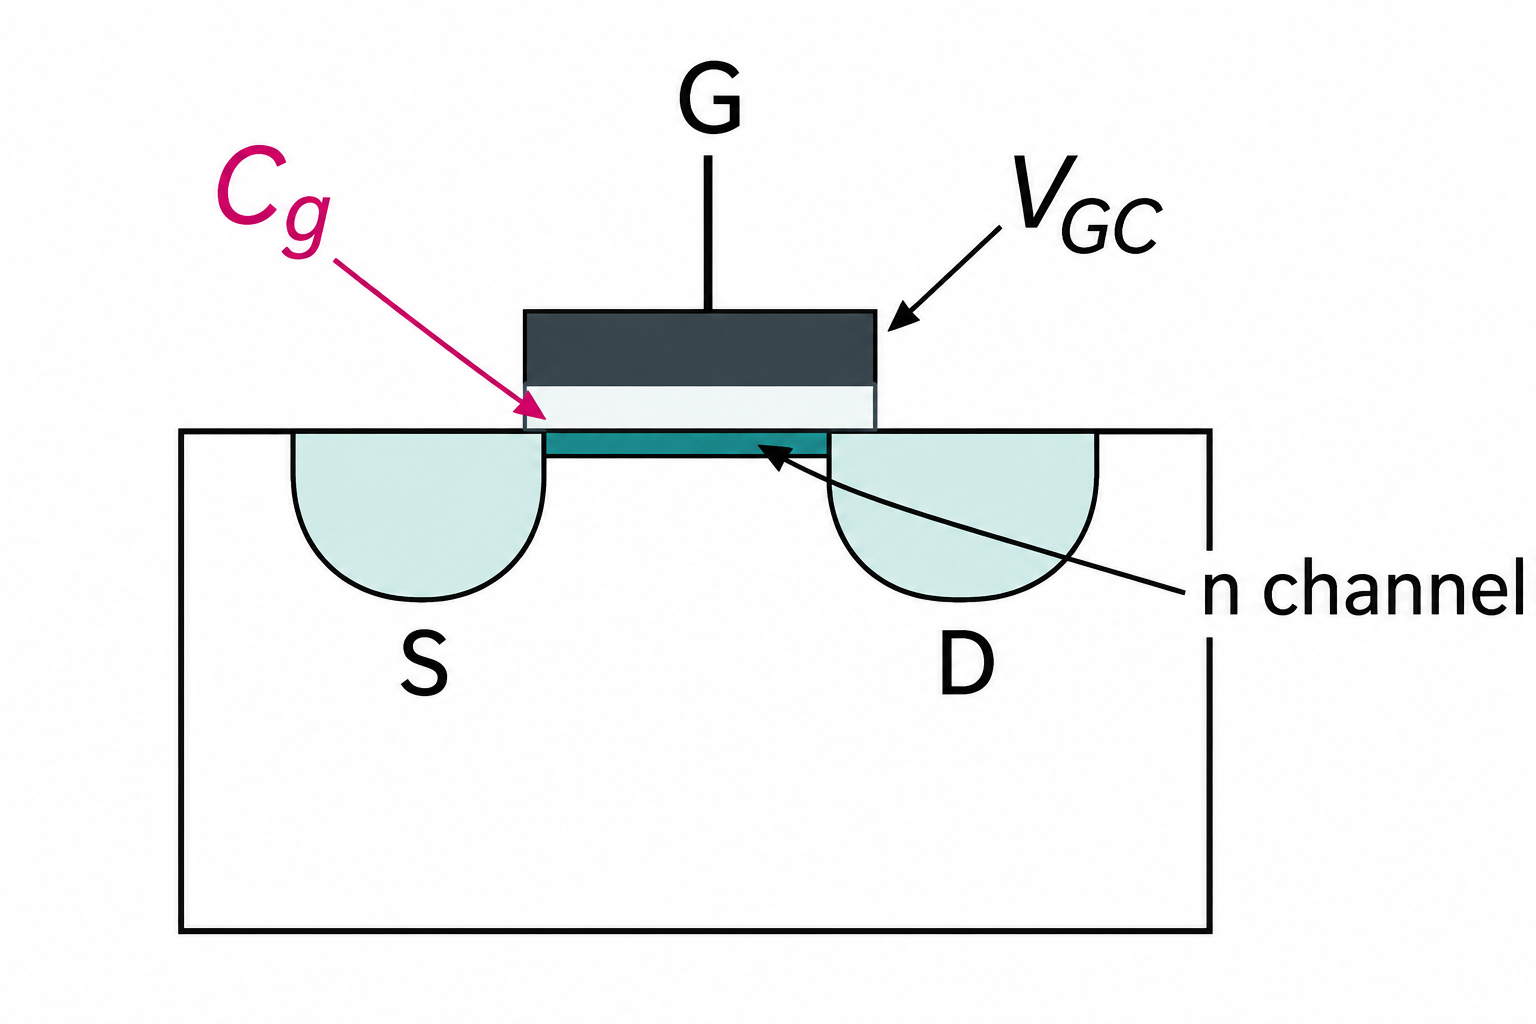
\includegraphics[width=0.4\linewidth,keepaspectratio]{figures/mosfet-gate-capacitance.png}
    \caption{Gate Capacitance of a Mosfet Device}
    \label{fig:}
\end{minipage}
\par\addvspace{7pt}
\keyequation{Voltage Between Gate and Channel}{V_{gc} = V_{gs} - \frac{V_{ds}}{2}}
\keyequation{Gate Capaictance}{C_{g} = C_{ox} W L}[
    \begin{itemize}
        \item $C_{ox}$ - Gate capaictance per micron equal to the premitivity of Silicon Oxide over the Oxide Thickness $\frac{\epsilon_0}{t_{ox}}$
        \item $W$ - Transistor Width
        \item $L$ - Channel Length
    \end{itemize}
]
\clearpage
\noteheading{1}{CMOS Inverter Transfer Characteristic}
\par\noindent\begin{minipage}{\linewidth}
    \begin{notesignal}[width=10.5cm,height=5.1cm,
        xmin=0,xmax=1.08,ymin=0,ymax=1.17,
        axis line style={NoteInk,line width=0.45pt,
            -{Latex[length=3pt,width=2pt]}},
        xtick={0,0.5,1},xticklabels={$0$,$V_{\mathrm{inv}}$,$V_{DD}$},
        ytick={1},yticklabels={$V_{DD}$},grid=none,
        xlabel={$V_{\mathrm{in}}$},ylabel={},
        xlabel style={at={(axis description cs:1,0)},anchor=west},
        enlargelimits=false,clip=false]{ }
        \node[above,font=\small] at (axis cs:0,1.17)
            {$V_{\mathrm{out}}$};
        \draw[NoteMuted,densely dashed,line width=0.4pt]
            (axis cs:0.5,0) -- (axis cs:0.5,0.5);
        % Balanced, ideal long-channel characteristic (normalized voltages).
        \addplot[NoteAccent,mark=none] coordinates {(0,1) (0.2,1)};
        \addplot[NoteAccent,mark=none,domain=0.2:0.5,samples=121]
            {x+0.2+sqrt(max(0,0.6*(1-2*x)))};
        \addplot[NoteAccent,mark=none]
            coordinates {(0.5,0.7) (0.5,0.3)};
        \addplot[NoteAccent,mark=none,domain=0.5:0.8,samples=121]
            {x-0.2-sqrt(max(0,0.6*(2*x-1)))};
        \addplot[NoteAccent,mark=none] coordinates {(0.8,0) (1,0)};
        \addplot[NoteAccent,only marks,mark=*,mark size=1.6pt]
            coordinates {(0.14,1) (0.425,0.925) (0.5,0.5)
                (0.575,0.075) (0.9,0)};
        \node[above=3pt,font=\small\sffamily,NoteAccent]
            at (axis cs:0.14,1) {A};
        \node[above left=3pt,font=\small\sffamily,NoteAccent]
            at (axis cs:0.425,0.925) {B};
        \node[left=4pt,font=\small\sffamily,NoteAccent]
            at (axis cs:0.5,0.5) {C};
        \node[above right=3pt,font=\small\sffamily,NoteAccent]
            at (axis cs:0.575,0.075) {D};
        \node[above=3pt,font=\small\sffamily,NoteAccent]
            at (axis cs:0.9,0) {E};
        \node[anchor=west,align=left,font=\scriptsize\sffamily,
            NoteMuted] at (axis cs:0.72,0.75)
            {Both transistors\\in saturation\\[2pt]
                $\dfrac{dV_{\mathrm{out}}}{dV_{\mathrm{in}}}\to-\infty$};
        \draw[NoteMuted,line width=0.3pt,
            -{Latex[length=2pt,width=1.4pt]}]
            (axis cs:0.71,0.64) -- (axis cs:0.52,0.52);
        \node[below=20pt,font=\small\sffamily,NoteMuted]
            at (axis cs:0.2,0) {Output 1};
        \node[below=20pt,font=\small\sffamily,NoteMuted]
            at (axis cs:0.8,0) {Output 0};
    \end{notesignal}
    \begin{center}
        \small $\beta_p=\beta_n,\quad V_{tn}=|V_{tp}|
            \quad\Longrightarrow\quad V_{\mathrm{inv}}=\dfrac{V_{DD}}{2}$
    \end{center}

    \begin{notederivation}{Inverter switching voltage}
        I_{DSn}&=-I_{DSp},\qquad
            V_{\mathrm{in}}=V_{\mathrm{out}}=V_{\mathrm{inv}}\\
        \frac{\beta_n}{2}(V_{\mathrm{inv}}-V_{tn})^2
            &=\frac{\beta_p}{2}(V_{DD}-V_{\mathrm{inv}}-|V_{tp}|)^2\\
        \sqrt{\frac{1}{\gamma}}(V_{\mathrm{inv}}-V_{tn})
            &=V_{DD}-V_{\mathrm{inv}}+V_{tp}\\
        V_{\mathrm{inv}}\left(1+\sqrt{\frac{1}{\gamma}}\right)
            &=V_{DD}+V_{tp}+V_{tn}\sqrt{\frac{1}{\gamma}}
    \end{notederivation}
    \keyequation{Inverter Switching Voltage}{
        V_{\mathrm{inv}}=
        \frac{V_{DD}+V_{tp}+V_{tn}\sqrt{\dfrac{1}{\gamma}}}
            {1+\sqrt{\dfrac{1}{\gamma}}}
    }

    \begingroup\small
    \begin{notetable}{lXl}{\textbf{Symbol} & \textbf{Meaning} & \textbf{Equation}}
        $V_{\mathrm{in}},V_{\mathrm{out}}$ & Input and output voltages & \\
        $V_{\mathrm{inv}}$ & Inverter switching voltage
            & $V_{\mathrm{in}}=V_{\mathrm{out}}=V_{\mathrm{inv}}$ \\
        $V_{DD}$ & Supply voltage & \\
        $V_{tn},V_{tp}$ & Signed NMOS and PMOS threshold voltages
            & $V_{tn}>0,\quad V_{tp}<0$ \\
        $\beta_n$ & NMOS transconductance parameter
            & $\beta_n=\mu_n C_{\mathrm{ox}}(W/L)_n$ \\
        $\beta_p$ & PMOS transconductance parameter
            & $\beta_p=\mu_p C_{\mathrm{ox}}(W/L)_p$ \\
        $\gamma$ & PMOS-to-NMOS strength ratio
            & $\gamma=\beta_p/\beta_n$ \\
        $I_{DSn},I_{DSp}$ & Signed NMOS and PMOS drain currents
            & $I_{DSn}=-I_{DSp}$ \\
    \end{notetable}
    \endgroup
\end{minipage}\par

For $V_{inv}$ to be in the middle, we want $\gamma = \frac{B_{p}}{B_{n}} = 1 \Rightarrow V_{inv} = V_{dd} \operatorname{if} V_{tp} = -V_{tn}$

\noteheading{1}{Noise Margin}

\par\addvspace{7pt}
\noindent\begin{minipage}{\linewidth}
    \centering
    \captionsetup{hypcap=false,type=figure}
    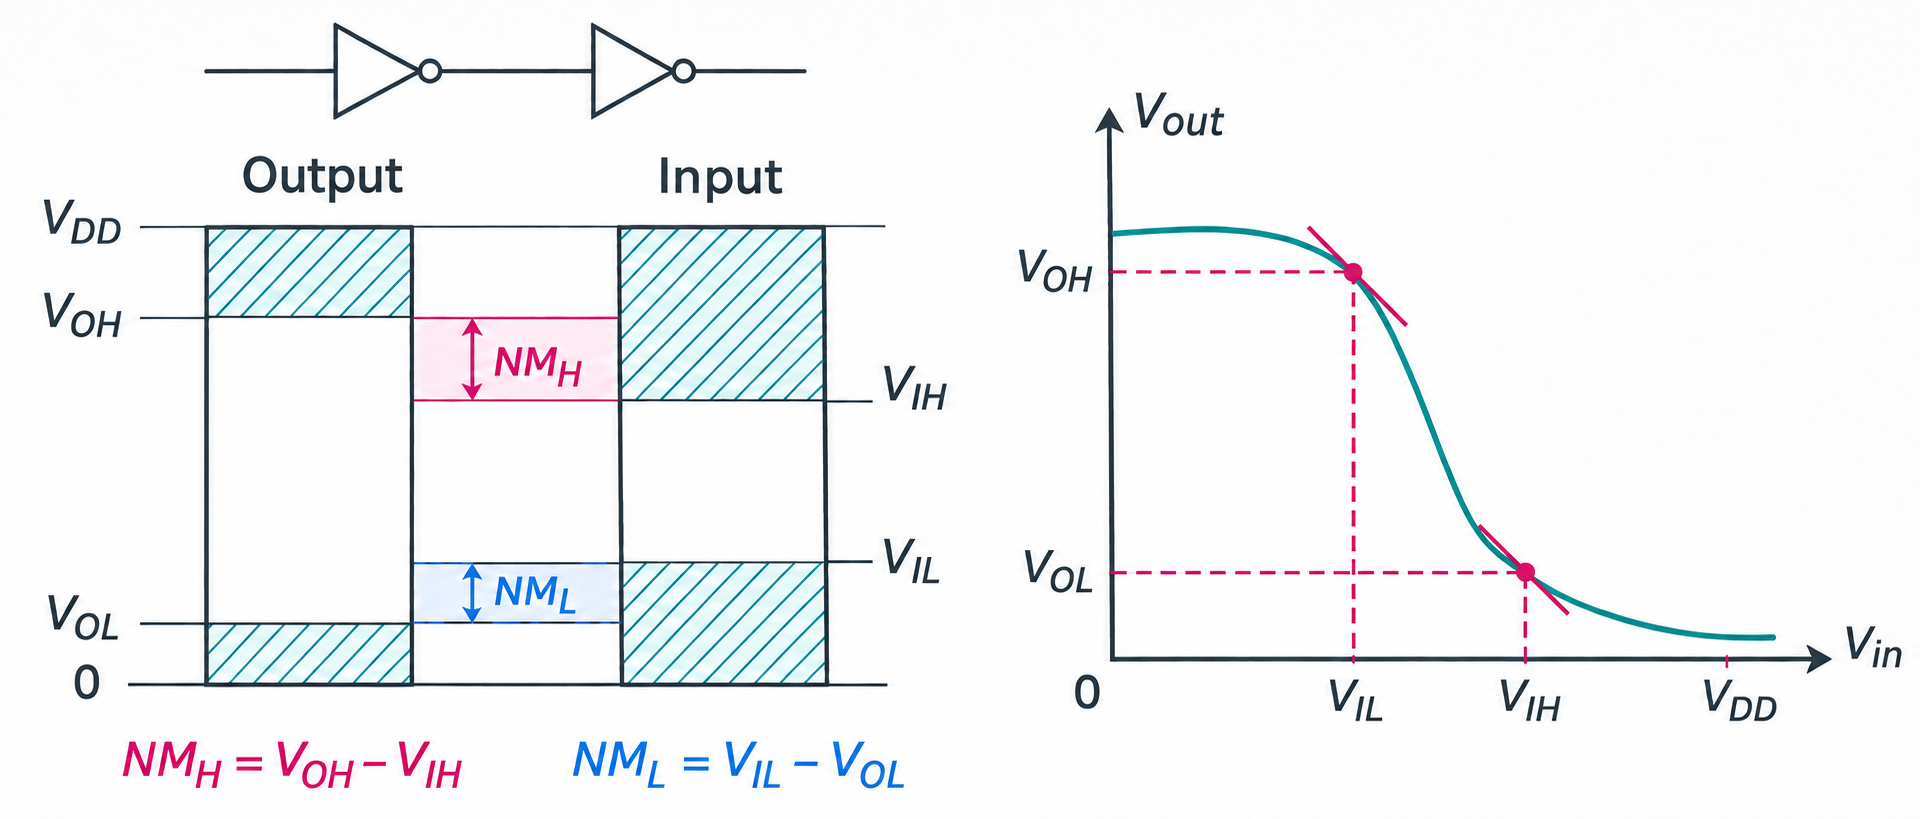
\includegraphics[width=0.8\linewidth,keepaspectratio]{figures/cmos-inverter-noise-margins.png}
    \caption{Noise Margin of an Inverter}
    \label{fig:}
\end{minipage}
\par\addvspace{7pt}

We want: $V_{OH} - V_{IH} = V_{IL} - V_{OL}$ (equalize the margin), that is the primary benefit of $\gamma = 1$. Other benefits of $\gamma = 1$ are:
\begin{itemize}
    \item Equalizes resistance of PMOS and NMOS
    \item Equalizes rise/fall time
\end{itemize}

\noteheading{2}{Performance due to Capacitance}
Performance of a CMOS circuit is equivalent to the R \& C values of the circuit.
\notedefinition{Performance of a CMOS Circuit}{Performance $\Rightarrow R \& C \because \text{delay} \propto RC$ }

\par\addvspace{7pt}
\noindent\begin{minipage}{\linewidth}
    \centering
    \captionsetup{hypcap=false,type=figure}
    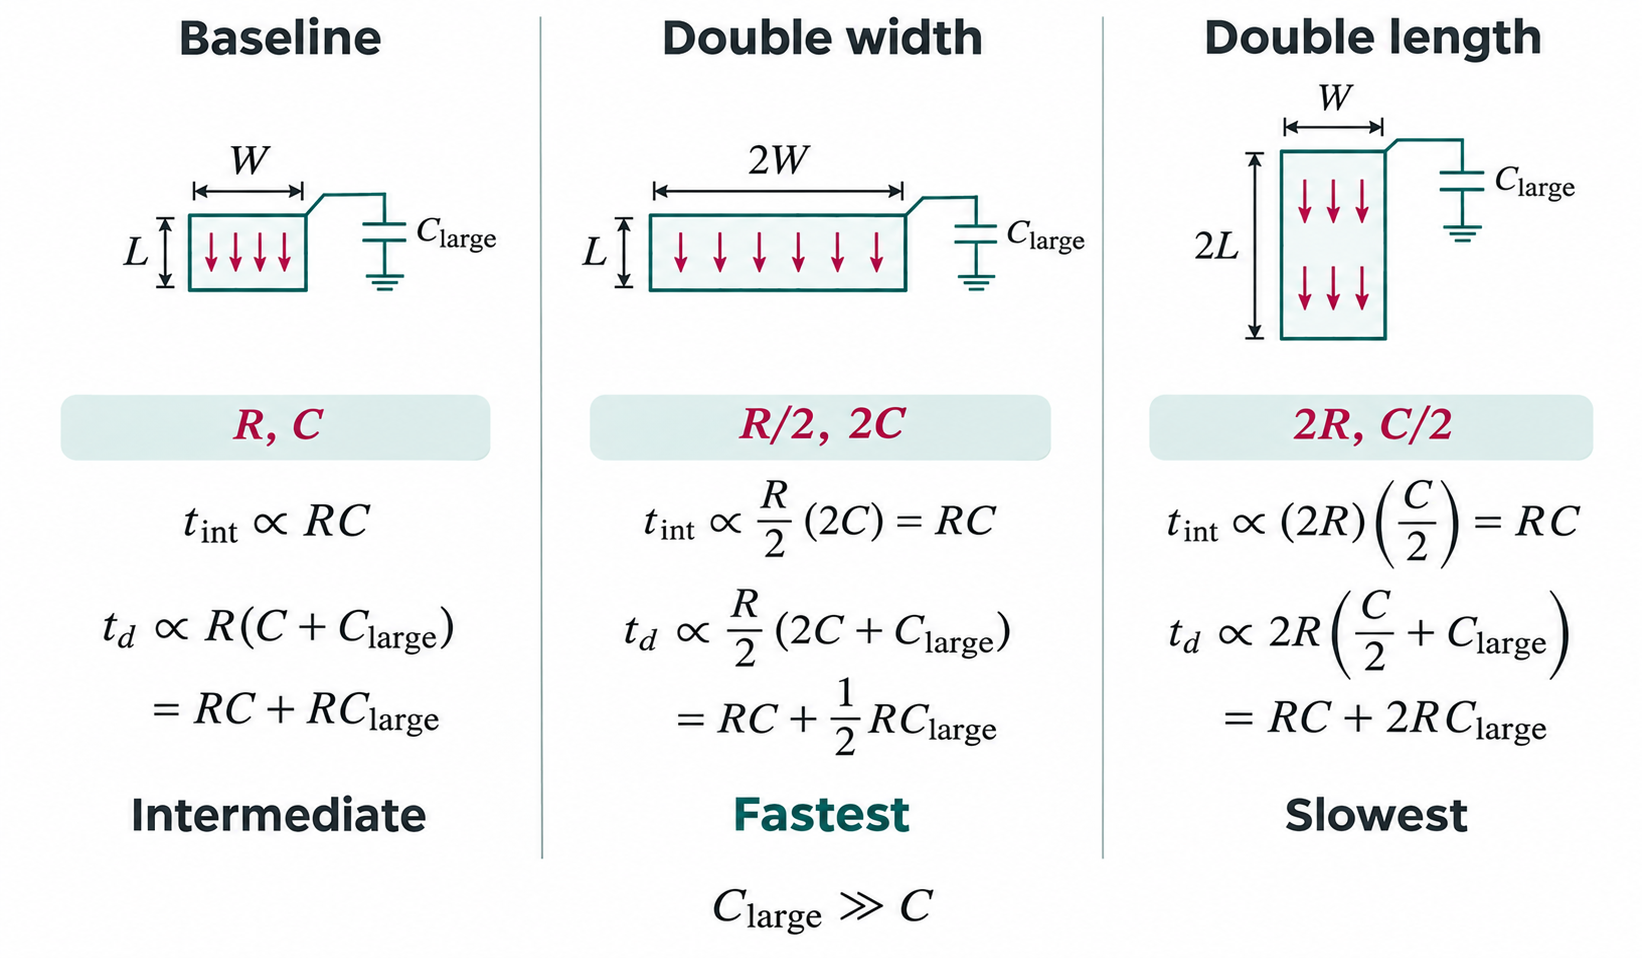
\includegraphics[width=0.8\linewidth,keepaspectratio]{figures/transistor-sizing-rc-delay.png}
    \caption{Transistor Sizing and RC Delay}
    \label{fig:}
\end{minipage}
\par\addvspace{7pt}

\noteheading{2}{C-V Characteristics}

$C_{g} = C_{ox} LW$ where $C_{OX} = 1 fF/ \mu m$ (valid for 9nm - 65nm processes)
\noteheading{3}{More Detailed Model of $C_{G}$}
\par\addvspace{7pt}
\noindent\begin{minipage}{\linewidth}
    \centering
    \captionsetup{hypcap=false,type=figure}
    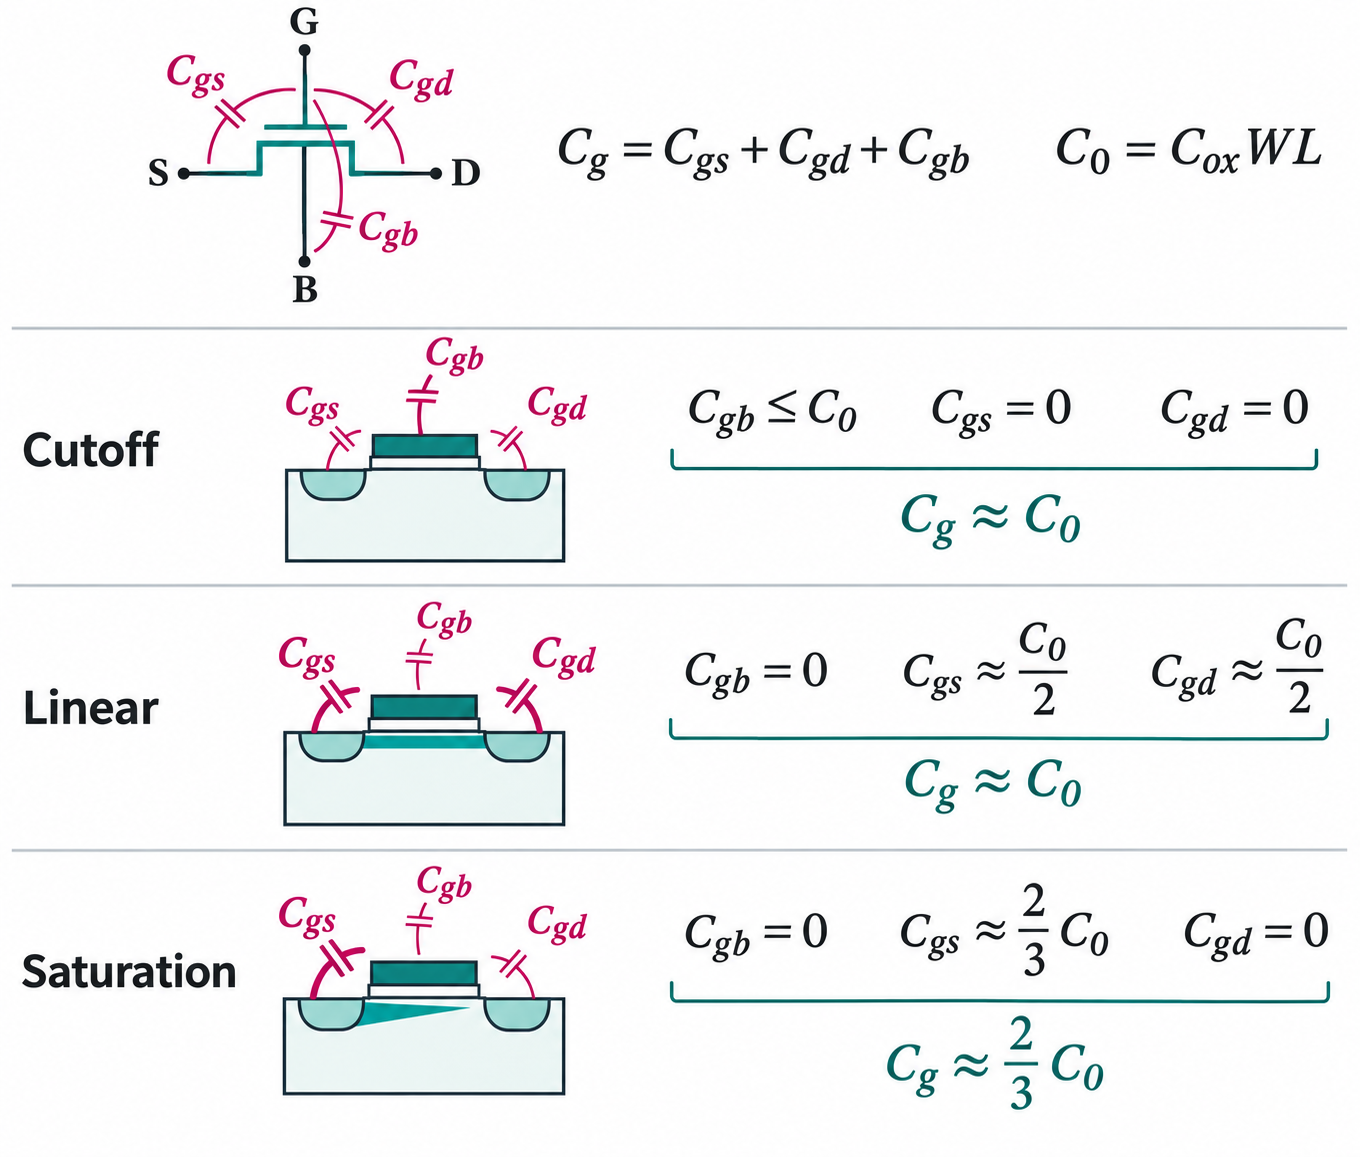
\includegraphics[width=0.8\linewidth,keepaspectratio]{figures/mosfet-gate-capacitance-regions.png}
    \caption{Capacitance Model at Different Regions of Operation}
    \label{fig:}
\end{minipage}
\par\addvspace{7pt}

\noteheading{4}{More on Gate Capacitance}
$C_{g}$ can be approximated as the output capacitance: $C_{g} = C_{gs} + C_{gd} + C_{b} \approx C_{o}$. Since foundaries typically overlap gates we have:
\keyequation{Gate Capaictance as a Function of Output Capacitance}{C_{g} = (C_{o} + 2C_{go_{1}}) \times w}[
    \begin{itemize}
        \item $C_o$ is output capacitance per micron
        \item $C_{go_{1}}$ is the overlap capacitance per micron
    \end{itemize}
]

\par\noindent\begin{minipage}{\linewidth}
\noteheading{3}{Diffusion Capacitance Model}

\par\addvspace{7pt}
\noindent\begin{minipage}{\linewidth}
    \centering
    \captionsetup{hypcap=false,type=figure}
    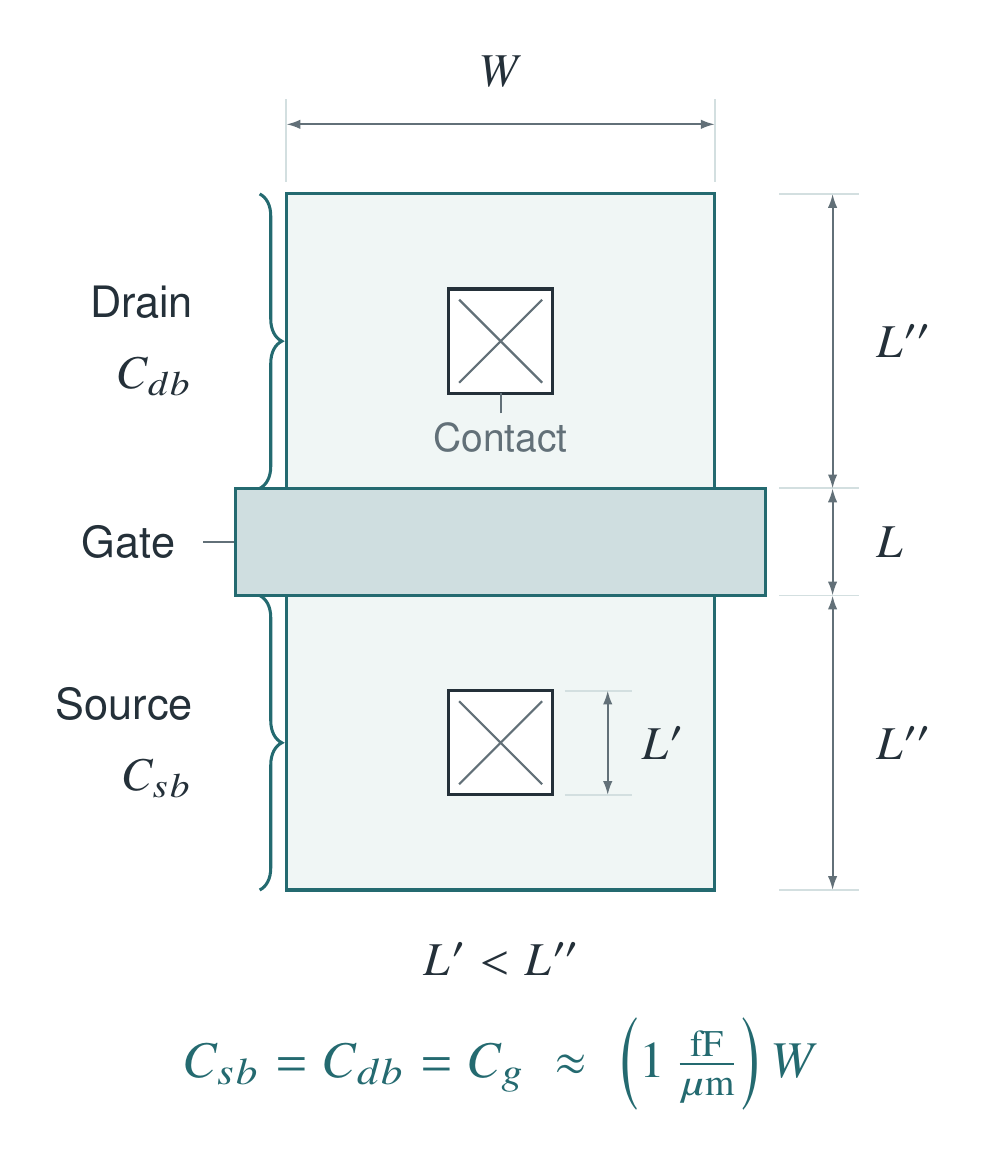
\includegraphics[width=0.4\linewidth,keepaspectratio]{figures/mosfet-layout-diffusion-capacitance.png}
    \caption{Diffusion Capacitance Model}
    \label{fig:}
\end{minipage}
\par\addvspace{7pt}

\keyequation{Diffusion Capacitance}{
    \begin{aligned}
        C_{sb} &= A_s C_{\mathrm{jbs}} + P_s C_{\mathrm{jbssw}} \\
        C_{\mathrm{jbs}} &= C_{\mathrm{jbd}} = C_{\mathrm{jb}} \\
        C_{\mathrm{jbssw}} &= C_{\mathrm{jbdsw}} = C_{\mathrm{jbsw}}
    \end{aligned}
}
\begingroup\small
\begin{notetable}{lXl}{\textbf{Symbol} & \textbf{Meaning} & \textbf{Unit}}
    $C_{sb}$ & Source-to-body diffusion capacitance & $\mathrm{fF}$ \\
    $A_s$ & Source diffusion area & $\mu\mathrm{m}^2$ \\
    $P_s$ & Source diffusion perimeter & $\mu\mathrm{m}$ \\
    $C_{\mathrm{jbs}},C_{\mathrm{jbd}},C_{\mathrm{jb}}$
        & Bottom junction capacitance per unit area & $\mathrm{fF}/\mu\mathrm{m}^2$ \\
    $C_{\mathrm{jbssw}},C_{\mathrm{jbdsw}},C_{\mathrm{jbsw}}$
        & Sidewall junction capacitance per unit length & $\mathrm{fF}/\mu\mathrm{m}$ \\
    $\mathrm{j}$ & Junction subscript & --- \\
    $\mathrm{sw}$ & Sidewall subscript & --- \\
\end{notetable}
\endgroup
\end{minipage}\par

\par\addvspace{7pt}
\noindent\begin{minipage}{\linewidth}
    \centering
    \captionsetup{hypcap=false,type=figure}
    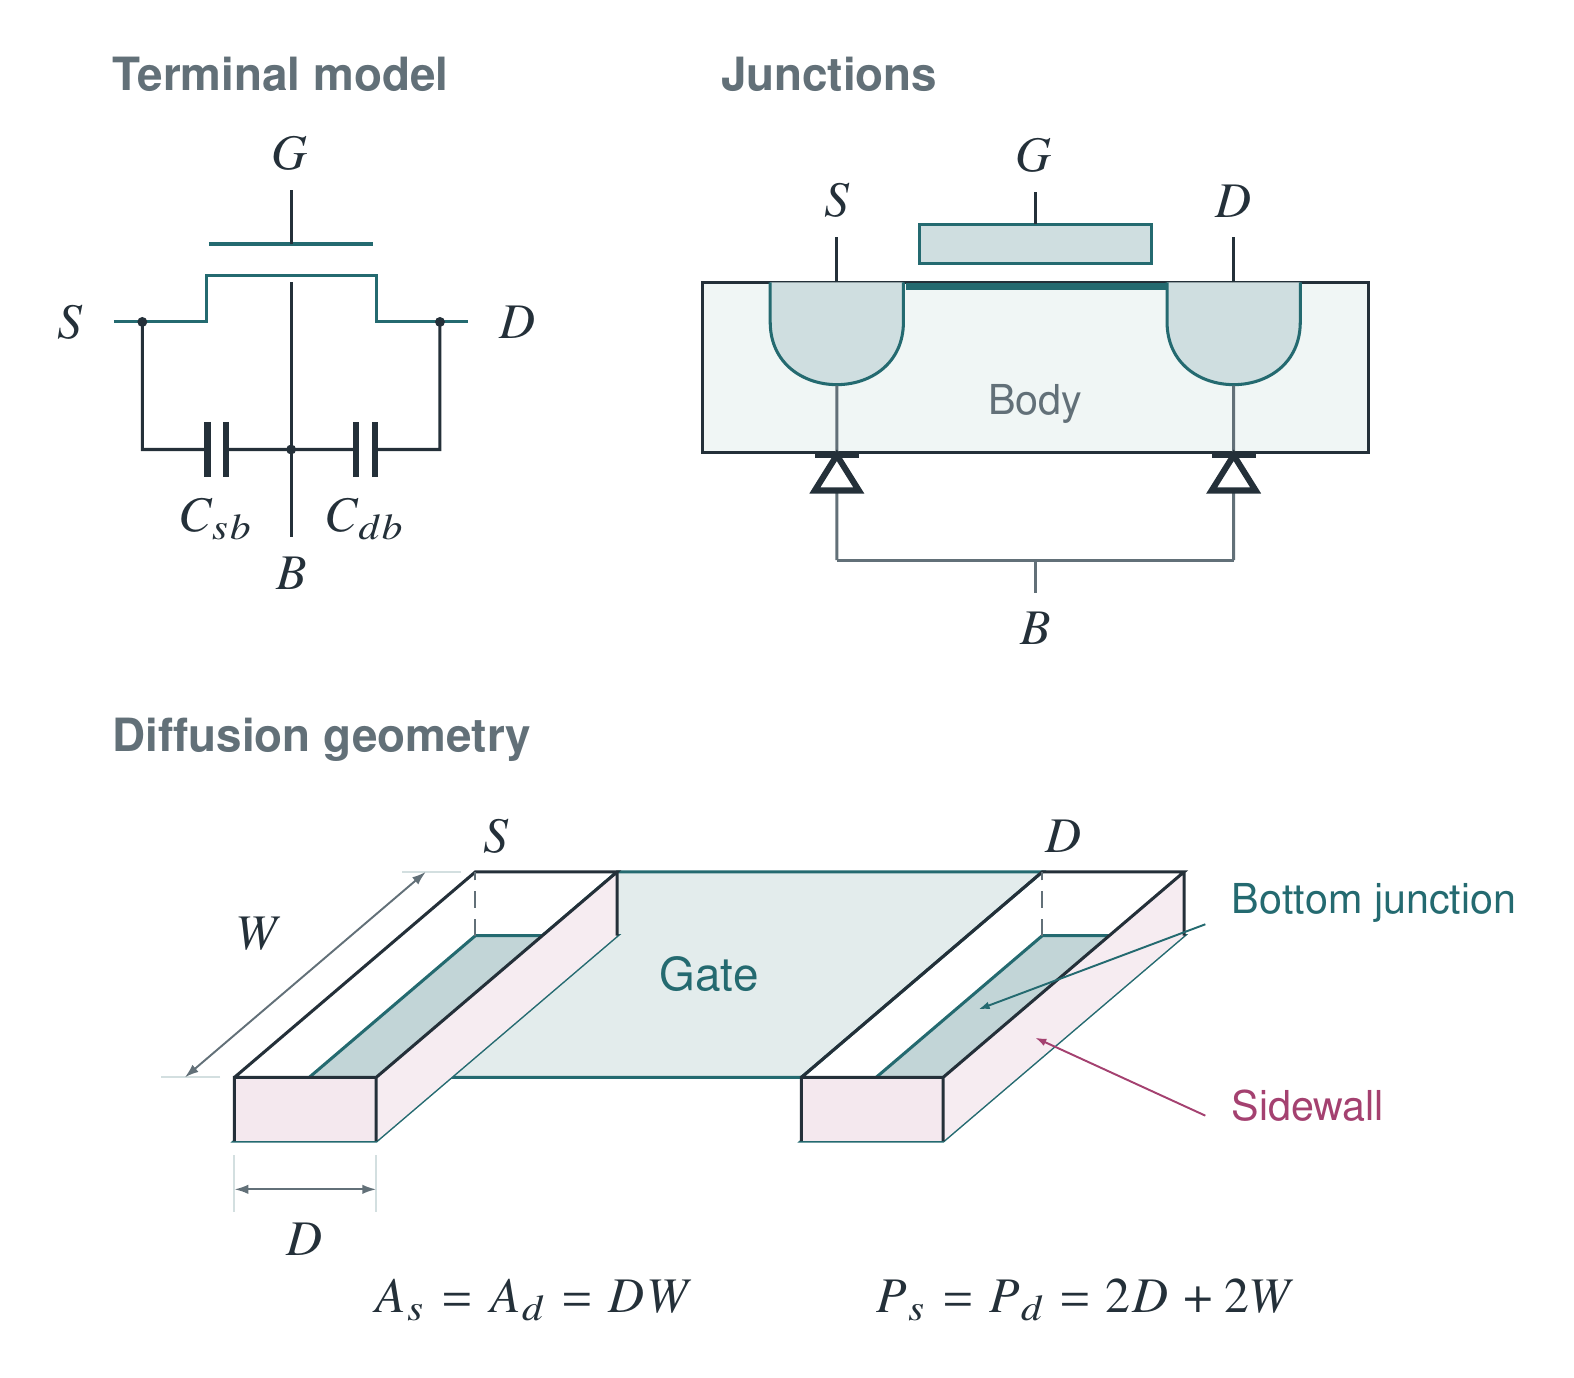
\includegraphics[width=0.8\linewidth,keepaspectratio]{figures/mosfet-junction-capacitance-geometry.png}
    \caption{Capacitance Model in 3-D}
    \label{fig:}
\end{minipage}
\par\addvspace{7pt}

\noteheading{1}{Voltage Threshhold Effect}
\par\addvspace{7pt}
\noindent\begin{minipage}{\linewidth}
    \centering
    \captionsetup{hypcap=false,type=figure}
    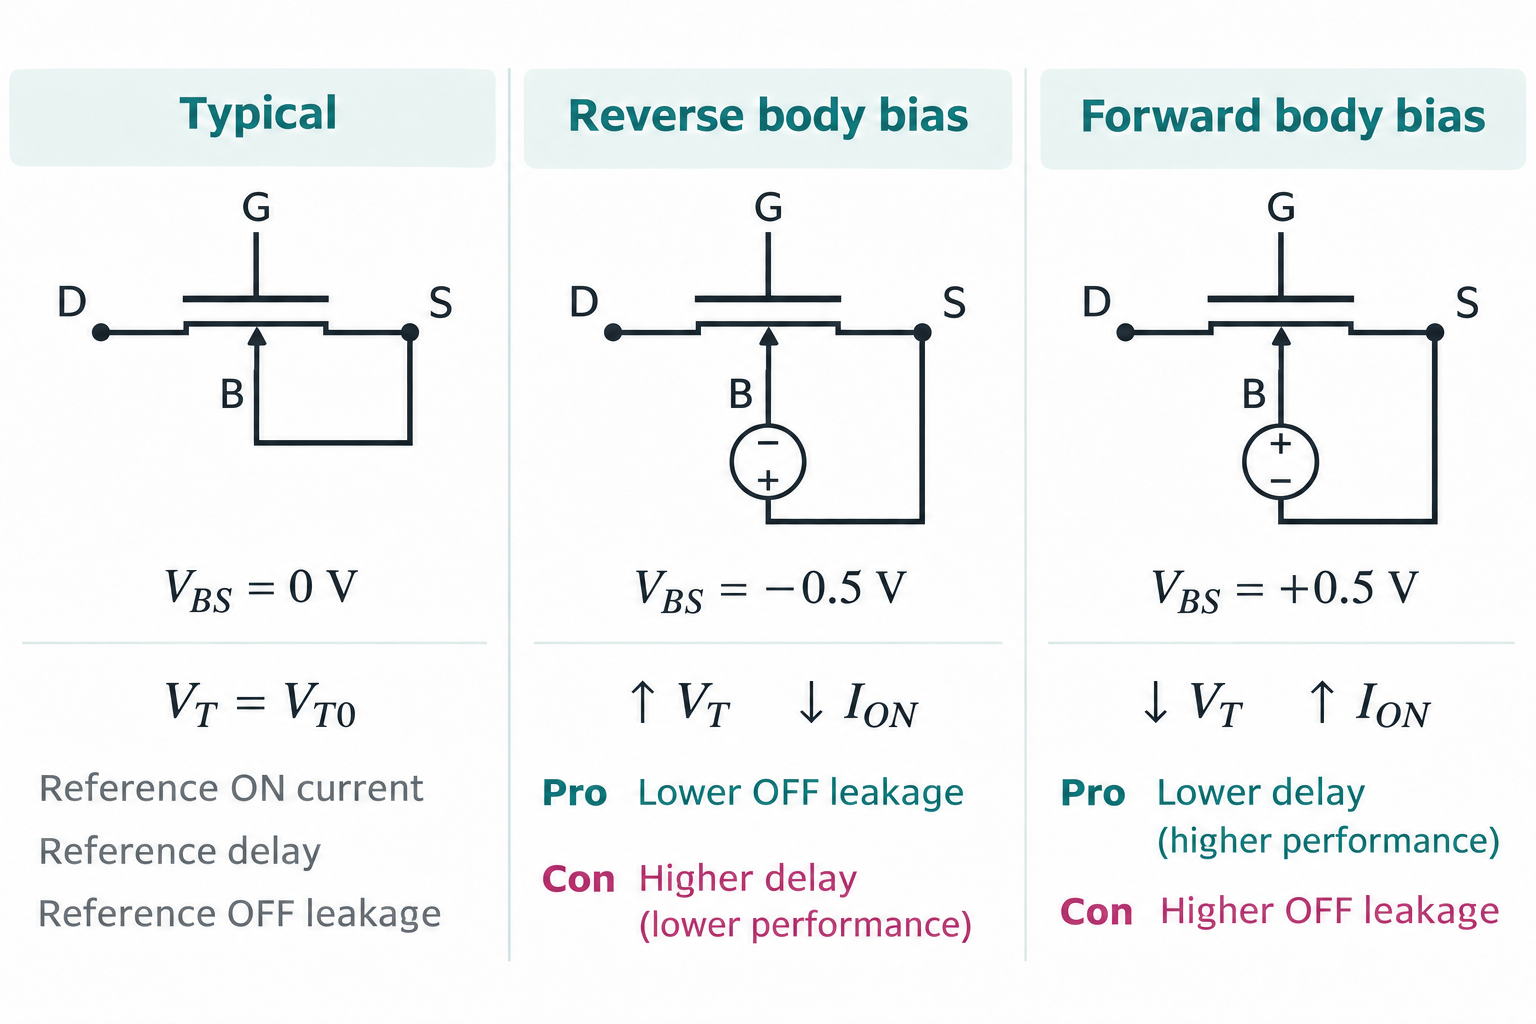
\includegraphics[width=0.65\linewidth,keepaspectratio]{figures/mosfet-body-bias-performance.png}
    \caption{Voltage Threshold and Performance}
    \label{fig:}
\end{minipage}
\keyequation{Threshold Voltage Equation}{V_{t} = V_{t_{0}} + \gamma (\sqrt{\phi_s + V_{sb}} - \sqrt{\phi_S})}[
    \begin{itemize}
        \item $\gamma$ - Body effect coefficient
        \item $V_{sb} \uparrow V_{t} \uparrow$
        \item $\Phi_S = 2V_T \frac{N_{A}}{\nu_i}$
    \end{itemize}
]

The relation is as follows:
\begin{itemize}
    \item $V_{t} \uparrow$ performance $\downarrow$ leakage (battery life, etc) $\downarrow$
    \item \item $V_{t} \downarrow$ performance $\uparrow$ leakage (battery life, etc) $\uparrow$
    \item With a variable $V_{SB}$ there is a trade-off between leakage and performance that needs to be considered
\end{itemize}

\noteheading{2}{Drain Induced Barrier Lowering (DIBL)}
$V_{t} = V_{t_{0}} - \nu V_{ds}$ where $\nu$ is the \textit{DIBL coefficient} and is equal to approximately: $0.1 V/V$. The DIBL equation is linearized from $V_{t_{0}}$

\par\noindent\begin{minipage}{\linewidth}
\noteheading{1}{Leakage Current}

\par\addvspace{7pt}
\noindent\begin{minipage}{\linewidth}
    \centering
    \captionsetup{hypcap=false,type=figure}
    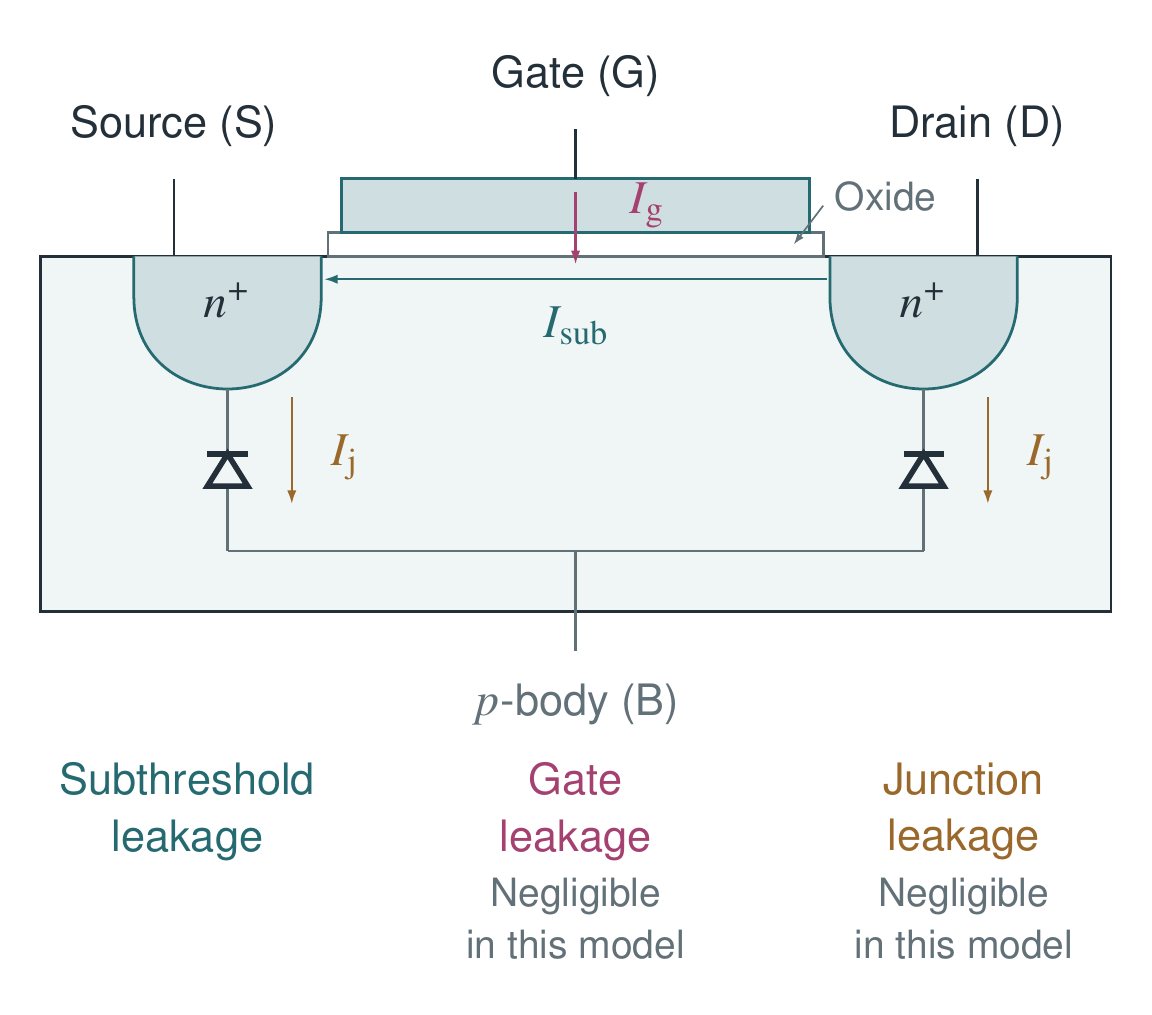
\includegraphics[width=0.8\linewidth,keepaspectratio]{figures/mosfet-leakage-mechanisms.png}
    \caption{}
    \label{fig:}
\end{minipage}
\par\addvspace{7pt}
\end{minipage}\par

\par\noindent\begin{minipage}{\linewidth}
\begin{notederivation}{Subthreshold leakage current}
    I_{\mathrm{sub}}
        &= I_{DS0}\exp\!\left(
            \frac{V_{GS}-V_{t0}+\eta V_{DS}-k_\gamma V_{SB}}{nV_T}
        \right)\left(1-e^{-V_{DS}/V_T}\right) \\
    I_{DS0} &= \beta V_T^2 e^{1.8},
        \qquad V_T=\frac{k_B T}{q} \\
    I_{\mathrm{ref}}
        &\equiv I_{DS0}\exp\!\left(
            \frac{-V_{t0}+\eta V_{DD}}{nV_T}
        \right) \\
    I_{\mathrm{sub}}
        &= I_{\mathrm{ref}}\exp\!\left(
            \frac{V_{GS}+\eta(V_{DS}-V_{DD})-k_\gamma V_{SB}}{nV_T}
        \right)\left(1-e^{-V_{DS}/V_T}\right)
\end{notederivation}
\notebox{Subthreshold notation}{
    \begingroup\small
    \setlength{\jot}{5pt}
    \[
    \begin{aligned}
    \log_{10}\!\left(
            \frac{I_{\mathrm{sub}}}
                {I_{\mathrm{ref}}\left(1-e^{-V_{DS}/V_T}\right)}
        \right)
        &= \frac{V_{GS}+\eta(V_{DS}-V_{DD})-k_\gamma V_{SB}}
            {nV_T\ln 10} \\
    \frac{\partial\log_{10} I_{\mathrm{sub}}}{\partial V_{GS}}
        &= \frac{1}{nV_T\ln 10} \\
    S &\equiv \left(
            \frac{\partial\log_{10} I_{\mathrm{sub}}}{\partial V_{GS}}
        \right)^{-1}
        = nV_T\ln 10
        \approx 100\,\mathrm{mV/dec}
    \end{aligned}
    \]
    \endgroup
}
\keyequation{Subthreshold Leakage Current}{
    I_{\mathrm{sub}}
        = I_{\mathrm{ref}}\,
        10^{\frac{V_{GS}+\eta(V_{DS}-V_{DD})-k_\gamma V_{SB}}{S}}
        \left(1-e^{-V_{DS}/V_T}\right)
}
\end{minipage}\par

\par\addvspace{12pt}
\noindent\begin{minipage}{\linewidth}
\begin{tcolorbox}[noteblock,colback=red!4,colframe=red!70!NoteInk,
    before skip=0pt,after skip=12pt,halign=center,
    fontupper=\sffamily\bfseries\boldmath\color{red!70!NoteInk}]
    Increase $V_{GS}-V_t$ by $100\,\mathrm{mV}$
    $\longrightarrow I_{\mathrm{sub}}\times 10$
\end{tcolorbox}
\begingroup\small
\begin{notetable}{lXX}{\textbf{Change} & \textbf{Subthreshold leakage} & \textbf{Saturation current and performance}}
    Dependence
        & $I_{\mathrm{sub}}\propto 10^{(V_{GS}-V_t)/S}$
        & $I_{DS}=\dfrac{\beta}{2}(V_{GS}-V_t)^2$ \\
    \midrule
    $V_{GS}\uparrow$
        & $I_{\mathrm{sub}}\uparrow$ exponentially; leakage power $\uparrow$
        & $I_{DS}\uparrow$ quadratically; performance $\uparrow$, delay $\downarrow$ \\
    $V_{GS}\downarrow$
        & $I_{\mathrm{sub}}\downarrow$ exponentially; leakage power $\downarrow$
        & $I_{DS}\downarrow$ quadratically; performance $\downarrow$, delay $\uparrow$ \\
    $V_t\uparrow$
        & $I_{\mathrm{sub}}\downarrow$ exponentially; leakage power $\downarrow$
        & $I_{DS}\downarrow$ quadratically; performance $\downarrow$, delay $\uparrow$ \\
    $V_t\downarrow$
        & $I_{\mathrm{sub}}\uparrow$ exponentially; leakage power $\uparrow$
        & $I_{DS}\uparrow$ quadratically; performance $\uparrow$, delay $\downarrow$ \\
\end{notetable}
{\footnotesize\color{NoteMuted}Other bias voltages and load held fixed.\par}
\endgroup
\end{minipage}\par

\noteheading{1}{Effect of Temperature on a Transistor}

\begin{align}
    \text{Temperature} \uparrow \Rightarrow &\downarrow \text{carrier mobility} \quad I_{DS, \text{saturation}} \downarrow \quad \text{performance} \downarrow \\
    &\downarrow V_{t} \quad I_{DS, \text{leakage}} \uparrow \quad \text{power consumption} \uparrow
\end{align}









\end{document}
